\documentclass[1p]{elsarticle_modified}
%\bibliographystyle{elsarticle-num}

%\usepackage[colorlinks]{hyperref}
%\usepackage{abbrmath_seonhwa} %\Abb, \Ascr, \Acal ,\Abf, \Afrak
\usepackage{amsfonts}
\usepackage{amssymb}
\usepackage{amsmath}
\usepackage{amsthm}
\usepackage{scalefnt}
\usepackage{amsbsy}
\usepackage{kotex}
\usepackage{caption}
\usepackage{subfig}
\usepackage{color}
\usepackage{graphicx}
\usepackage{xcolor} %% white, black, red, green, blue, cyan, magenta, yellow
\usepackage{float}
\usepackage{setspace}
\usepackage{hyperref}

\usepackage{tikz}
\usetikzlibrary{arrows}

\usepackage{multirow}
\usepackage{array} % fixed length table
\usepackage{hhline}

%%%%%%%%%%%%%%%%%%%%%
\makeatletter
\renewcommand*\env@matrix[1][\arraystretch]{%
	\edef\arraystretch{#1}%
	\hskip -\arraycolsep
	\let\@ifnextchar\new@ifnextchar
	\array{*\c@MaxMatrixCols c}}
\makeatother %https://tex.stackexchange.com/questions/14071/how-can-i-increase-the-line-spacing-in-a-matrix
%%%%%%%%%%%%%%%

\usepackage[normalem]{ulem}

\newcommand{\msout}[1]{\ifmmode\text{\sout{\ensuremath{#1}}}\else\sout{#1}\fi}
%SOURCE: \msout is \stkout macro in https://tex.stackexchange.com/questions/20609/strikeout-in-math-mode

\newcommand{\cancel}[1]{
	\ifmmode
	{\color{red}\msout{#1}}
	\else
	{\color{red}\sout{#1}}
	\fi
}

\newcommand{\add}[1]{
	{\color{blue}\uwave{#1}}
}

\newcommand{\replace}[2]{
	\ifmmode
	{\color{red}\msout{#1}}{\color{blue}\uwave{#2}}
	\else
	{\color{red}\sout{#1}}{\color{blue}\uwave{#2}}
	\fi
}

\newcommand{\Sol}{\mathcal{S}} %segment
\newcommand{\D}{D} %diagram
\newcommand{\A}{\mathcal{A}} %arc


%%%%%%%%%%%%%%%%%%%%%%%%%%%%%5 test

\def\sl{\operatorname{\textup{SL}}(2,\Cbb)}
\def\psl{\operatorname{\textup{PSL}}(2,\Cbb)}
\def\quan{\mkern 1mu \triangleright \mkern 1mu}

\theoremstyle{definition}
\newtheorem{thm}{Theorem}[section]
\newtheorem{prop}[thm]{Proposition}
\newtheorem{lem}[thm]{Lemma}
\newtheorem{ques}[thm]{Question}
\newtheorem{cor}[thm]{Corollary}
\newtheorem{defn}[thm]{Definition}
\newtheorem{exam}[thm]{Example}
\newtheorem{rmk}[thm]{Remark}
\newtheorem{alg}[thm]{Algorithm}

\newcommand{\I}{\sqrt{-1}}
\begin{document}

%\begin{frontmatter}
%
%\title{Boundary parabolic representations of knots up to 8 crossings}
%
%%% Group authors per affiliation:
%\author{Yunhi Cho} 
%\address{Department of Mathematics, University of Seoul, Seoul, Korea}
%\ead{yhcho@uos.ac.kr}
%
%
%\author{Seonhwa Kim} %\fnref{s_kim}}
%\address{Center for Geometry and Physics, Institute for Basic Science, Pohang, 37673, Korea}
%\ead{ryeona17@ibs.re.kr}
%
%\author{Hyuk Kim}
%\address{Department of Mathematical Sciences, Seoul National University, Seoul 08826, Korea}
%\ead{hyukkim@snu.ac.kr}
%
%\author{Seokbeom Yoon}
%\address{Department of Mathematical Sciences, Seoul National University, Seoul, 08826,  Korea}
%\ead{sbyoon15@snu.ac.kr}
%
%\begin{abstract}
%We find all boundary parabolic representation of knots up to 8 crossings.
%
%\end{abstract}
%\begin{keyword}
%    \MSC[2010] 57M25 
%\end{keyword}
%
%\end{frontmatter}

%\linenumbers
%\tableofcontents
%
\newcommand\colored[1]{\textcolor{white}{\rule[-0.35ex]{0.8em}{1.4ex}}\kern-0.8em\color{red} #1}%
%\newcommand\colored[1]{\textcolor{white}{ #1}\kern-2.17ex	\textcolor{white}{ #1}\kern-1.81ex	\textcolor{white}{ #1}\kern-2.15ex\color{red}#1	}

{\Large $\underline{12a_{0726}~(K12a_{0726})}$}

\setlength{\tabcolsep}{10pt}
\renewcommand{\arraystretch}{1.6}
\vspace{1cm}\begin{tabular}{m{100pt}>{\centering\arraybackslash}m{274pt}}
\multirow{5}{120pt}{
	\centering
	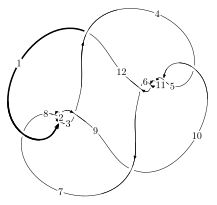
\includegraphics[width=112pt]{../../../GIT/diagram.site/Diagrams/png/1527_12a_0726.png}\\
\ \ \ A knot diagram\footnotemark}&
\allowdisplaybreaks
\textbf{Linearized knot diagam} \\
\cline{2-2}
 &
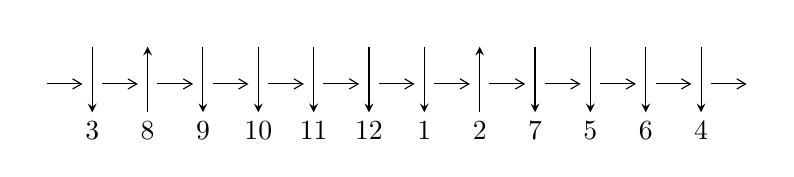
\begin{tikzpicture}[x=20pt, y=17pt]
	% nodes
	\node (C0) at (0, 0) {};
	\node (C1) at (1, 0) {};
	\node (C1U) at (1, +1) {};
	\node (C1D) at (1, -1) {3};

	\node (C2) at (2, 0) {};
	\node (C2U) at (2, +1) {};
	\node (C2D) at (2, -1) {8};

	\node (C3) at (3, 0) {};
	\node (C3U) at (3, +1) {};
	\node (C3D) at (3, -1) {9};

	\node (C4) at (4, 0) {};
	\node (C4U) at (4, +1) {};
	\node (C4D) at (4, -1) {10};

	\node (C5) at (5, 0) {};
	\node (C5U) at (5, +1) {};
	\node (C5D) at (5, -1) {11};

	\node (C6) at (6, 0) {};
	\node (C6U) at (6, +1) {};
	\node (C6D) at (6, -1) {12};

	\node (C7) at (7, 0) {};
	\node (C7U) at (7, +1) {};
	\node (C7D) at (7, -1) {1};

	\node (C8) at (8, 0) {};
	\node (C8U) at (8, +1) {};
	\node (C8D) at (8, -1) {2};

	\node (C9) at (9, 0) {};
	\node (C9U) at (9, +1) {};
	\node (C9D) at (9, -1) {7};

	\node (C10) at (10, 0) {};
	\node (C10U) at (10, +1) {};
	\node (C10D) at (10, -1) {5};

	\node (C11) at (11, 0) {};
	\node (C11U) at (11, +1) {};
	\node (C11D) at (11, -1) {6};

	\node (C12) at (12, 0) {};
	\node (C12U) at (12, +1) {};
	\node (C12D) at (12, -1) {4};
	\node (C13) at (13, 0) {};

	% arrows
	\draw[->,>={angle 60}]
	(C0) edge (C1) (C1) edge (C2) (C2) edge (C3) (C3) edge (C4) (C4) edge (C5) (C5) edge (C6) (C6) edge (C7) (C7) edge (C8) (C8) edge (C9) (C9) edge (C10) (C10) edge (C11) (C11) edge (C12) (C12) edge (C13) ;	\draw[->,>=stealth]
	(C1U) edge (C1D) (C2D) edge (C2U) (C3U) edge (C3D) (C4U) edge (C4D) (C5U) edge (C5D) (C6U) edge (C6D) (C7U) edge (C7D) (C8D) edge (C8U) (C9U) edge (C9D) (C10U) edge (C10D) (C11U) edge (C11D) (C12U) edge (C12D) ;
	\end{tikzpicture} \\
\hhline{~~} \\& 
\textbf{Solving Sequence} \\ \cline{2-2} 
 &
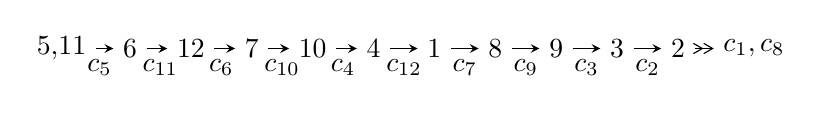
\begin{tikzpicture}[x=22pt, y=7pt]
	% node
	\node (A0) at (-1/8, 0) {5,11};
	\node (A1) at (1, 0) {6};
	\node (A2) at (2, 0) {12};
	\node (A3) at (3, 0) {7};
	\node (A4) at (4, 0) {10};
	\node (A5) at (5, 0) {4};
	\node (A6) at (6, 0) {1};
	\node (A7) at (7, 0) {8};
	\node (A8) at (8, 0) {9};
	\node (A9) at (9, 0) {3};
	\node (A10) at (10, 0) {2};
	\node (C1) at (1/2, -1) {$c_{5}$};
	\node (C2) at (3/2, -1) {$c_{11}$};
	\node (C3) at (5/2, -1) {$c_{6}$};
	\node (C4) at (7/2, -1) {$c_{10}$};
	\node (C5) at (9/2, -1) {$c_{4}$};
	\node (C6) at (11/2, -1) {$c_{12}$};
	\node (C7) at (13/2, -1) {$c_{7}$};
	\node (C8) at (15/2, -1) {$c_{9}$};
	\node (C9) at (17/2, -1) {$c_{3}$};
	\node (C10) at (19/2, -1) {$c_{2}$};
	\node (A11) at (45/4, 0) {$c_{1},c_{8}$};

	% edge
	\draw[->,>=stealth]	
	(A0) edge (A1) (A1) edge (A2) (A2) edge (A3) (A3) edge (A4) (A4) edge (A5) (A5) edge (A6) (A6) edge (A7) (A7) edge (A8) (A8) edge (A9) (A9) edge (A10) ;
	\draw[->>,>={angle 60}]	
	(A10) edge (A11);
\end{tikzpicture} \\ 

\end{tabular} \\

\footnotetext{
The image of knot diagram is generated by the software ``\textbf{Draw programme}" developed by Andrew Bartholomew(\url{http://www.layer8.co.uk/maths/draw/index.htm\#Running-draw}), where we modified some parts for our purpose(\url{https://github.com/CATsTAILs/LinksPainter}).
}\phantom \\ \newline 
\centering \textbf{Ideals for irreducible components\footnotemark of $X_{\text{par}}$} 
 
\begin{align*}
I^u_{1}&=\langle 
u^{51}- u^{50}+\cdots-2 u-1\rangle \\
\\
\end{align*}
\raggedright * 1 irreducible components of $\dim_{\mathbb{C}}=0$, with total 51 representations.\\
\footnotetext{All coefficients of polynomials are rational numbers. But the coefficients are sometimes approximated in decimal forms when there is not enough margin.}
\newpage
\renewcommand{\arraystretch}{1}
\centering \section*{I. $I^u_{1}= \langle u^{51}- u^{50}+\cdots-2 u-1 \rangle$}
\flushleft \textbf{(i) Arc colorings}\\
\begin{tabular}{m{7pt} m{180pt} m{7pt} m{180pt} }
\flushright $a_{5}=$&$\begin{pmatrix}1\\0\end{pmatrix}$ \\
\flushright $a_{11}=$&$\begin{pmatrix}0\\u\end{pmatrix}$ \\
\flushright $a_{6}=$&$\begin{pmatrix}1\\u^2\end{pmatrix}$ \\
\flushright $a_{12}=$&$\begin{pmatrix}- u\\- u^3+u\end{pmatrix}$ \\
\flushright $a_{7}=$&$\begin{pmatrix}- u^2+1\\- u^4+2 u^2\end{pmatrix}$ \\
\flushright $a_{10}=$&$\begin{pmatrix}u\\u\end{pmatrix}$ \\
\flushright $a_{4}=$&$\begin{pmatrix}- u^2+1\\- u^2\end{pmatrix}$ \\
\flushright $a_{1}=$&$\begin{pmatrix}u^7-4 u^5+4 u^3-2 u\\u^7-3 u^5+u\end{pmatrix}$ \\
\flushright $a_{8}=$&$\begin{pmatrix}u^{18}-11 u^{16}+48 u^{14}-107 u^{12}+133 u^{10}-95 u^8+34 u^6-2 u^4-3 u^2+1\\u^{18}-10 u^{16}+37 u^{14}-60 u^{12}+35 u^{10}+8 u^8-16 u^6+2 u^4+3 u^2\end{pmatrix}$ \\
\flushright $a_{9}=$&$\begin{pmatrix}- u^7+4 u^5-4 u^3+2 u\\- u^9+5 u^7-7 u^5+2 u^3+u\end{pmatrix}$ \\
\flushright $a_{3}=$&$\begin{pmatrix}u^{18}-11 u^{16}+48 u^{14}-107 u^{12}+133 u^{10}-95 u^8+34 u^6-2 u^4-3 u^2+1\\u^{20}-12 u^{18}+\cdots-5 u^4-2 u^2\end{pmatrix}$ \\
\flushright $a_{2}=$&$\begin{pmatrix}u^{45}-28 u^{43}+\cdots+14 u^3-3 u\\u^{47}-29 u^{45}+\cdots+2 u^3+u\end{pmatrix}$\\&\end{tabular}
\flushleft \textbf{(ii) Obstruction class $= -1$}\\~\\
\flushleft \textbf{(iii) Cusp Shapes $= 4 u^{47}-120 u^{45}+\cdots-16 u-14$}\\~\\
\newpage\renewcommand{\arraystretch}{1}
\flushleft \textbf{(iv) u-Polynomials at the component}\newline \\
\begin{tabular}{m{50pt}|m{274pt}}
Crossings & \hspace{64pt}u-Polynomials at each crossing \\
\hline $$\begin{aligned}c_{1}\end{aligned}$$&$\begin{aligned}
&u^{51}+27 u^{50}+\cdots+2 u-1
\end{aligned}$\\
\hline $$\begin{aligned}c_{2},c_{8}\end{aligned}$$&$\begin{aligned}
&u^{51}- u^{50}+\cdots+u^2-1
\end{aligned}$\\
\hline $$\begin{aligned}c_{3},c_{7}\end{aligned}$$&$\begin{aligned}
&u^{51}+u^{50}+\cdots-40 u-13
\end{aligned}$\\
\hline $$\begin{aligned}c_{4},c_{5},c_{6}\\c_{10},c_{11}\end{aligned}$$&$\begin{aligned}
&u^{51}- u^{50}+\cdots-2 u-1
\end{aligned}$\\
\hline $$\begin{aligned}c_{9},c_{12}\end{aligned}$$&$\begin{aligned}
&u^{51}-5 u^{50}+\cdots+42 u+5
\end{aligned}$\\
\hline
\end{tabular}\\~\\
\newpage\renewcommand{\arraystretch}{1}
\flushleft \textbf{(v) Riley Polynomials at the component}\newline \\
\begin{tabular}{m{50pt}|m{274pt}}
Crossings & \hspace{64pt}Riley Polynomials at each crossing \\
\hline $$\begin{aligned}c_{1}\end{aligned}$$&$\begin{aligned}
&y^{51}-5 y^{50}+\cdots+34 y-1
\end{aligned}$\\
\hline $$\begin{aligned}c_{2},c_{8}\end{aligned}$$&$\begin{aligned}
&y^{51}+27 y^{50}+\cdots+2 y-1
\end{aligned}$\\
\hline $$\begin{aligned}c_{3},c_{7}\end{aligned}$$&$\begin{aligned}
&y^{51}-37 y^{50}+\cdots+4018 y-169
\end{aligned}$\\
\hline $$\begin{aligned}c_{4},c_{5},c_{6}\\c_{10},c_{11}\end{aligned}$$&$\begin{aligned}
&y^{51}-65 y^{50}+\cdots+2 y-1
\end{aligned}$\\
\hline $$\begin{aligned}c_{9},c_{12}\end{aligned}$$&$\begin{aligned}
&y^{51}+23 y^{50}+\cdots+974 y-25
\end{aligned}$\\
\hline
\end{tabular}\\~\\
\newpage\flushleft \textbf{(vi) Complex Volumes and Cusp Shapes}
$$\begin{array}{c|c|c}  
\text{Solutions to }I^u_{1}& \I (\text{vol} + \sqrt{-1}CS) & \text{Cusp shape}\\
 \hline 
\begin{aligned}
u &= -0.934654 + 0.359124 I\end{aligned}
 & -4.89993 + 10.88520 I & -13.9898 - 9.1011 I \\ \hline\begin{aligned}
u &= -0.934654 - 0.359124 I\end{aligned}
 & -4.89993 - 10.88520 I & -13.9898 + 9.1011 I \\ \hline\begin{aligned}
u &= -0.942251 + 0.324875 I\end{aligned}
 & -5.98706 + 2.32675 I & -15.9409 - 2.8840 I \\ \hline\begin{aligned}
u &= -0.942251 - 0.324875 I\end{aligned}
 & -5.98706 - 2.32675 I & -15.9409 + 2.8840 I \\ \hline\begin{aligned}
u &= \phantom{-}0.922701 + 0.345886 I\end{aligned}
 & -1.94667 - 6.07625 I & -10.83807 + 6.02977 I \\ \hline\begin{aligned}
u &= \phantom{-}0.922701 - 0.345886 I\end{aligned}
 & -1.94667 + 6.07625 I & -10.83807 - 6.02977 I \\ \hline\begin{aligned}
u &= \phantom{-}1.03108\phantom{ +0.000000I}\end{aligned}
 & -5.66531\phantom{ +0.000000I} & -15.3850\phantom{ +0.000000I} \\ \hline\begin{aligned}
u &= -1.061590 + 0.031424 I\end{aligned}
 & -9.08913 + 4.30907 I & -18.5429 - 3.7969 I \\ \hline\begin{aligned}
u &= -1.061590 - 0.031424 I\end{aligned}
 & -9.08913 - 4.30907 I & -18.5429 + 3.7969 I \\ \hline\begin{aligned}
u &= \phantom{-}0.855219 + 0.348235 I\end{aligned}
 & \phantom{-}0.95095 - 5.30967 I & -8.63248 + 7.99988 I \\ \hline\begin{aligned}
u &= \phantom{-}0.855219 - 0.348235 I\end{aligned}
 & \phantom{-}0.95095 + 5.30967 I & -8.63248 - 7.99988 I \\ \hline\begin{aligned}
u &= \phantom{-}0.892740 + 0.163983 I\end{aligned}
 & -3.77255 - 2.37268 I & -17.3684 + 5.1349 I \\ \hline\begin{aligned}
u &= \phantom{-}0.892740 - 0.163983 I\end{aligned}
 & -3.77255 + 2.37268 I & -17.3684 - 5.1349 I \\ \hline\begin{aligned}
u &= -0.812894 + 0.338645 I\end{aligned}
 & \phantom{-}1.22174 + 0.86320 I & -7.59219 - 0.99621 I \\ \hline\begin{aligned}
u &= -0.812894 - 0.338645 I\end{aligned}
 & \phantom{-}1.22174 - 0.86320 I & -7.59219 + 0.99621 I \\ \hline\begin{aligned}
u &= -0.691855 + 0.295789 I\end{aligned}
 & -0.586592 - 0.013554 I & -8.91489 - 1.65499 I \\ \hline\begin{aligned}
u &= -0.691855 - 0.295789 I\end{aligned}
 & -0.586592 + 0.013554 I & -8.91489 + 1.65499 I \\ \hline\begin{aligned}
u &= \phantom{-}0.657710 + 0.357951 I\end{aligned}
 & -3.33920 + 4.49491 I & -12.31496 - 1.64994 I \\ \hline\begin{aligned}
u &= \phantom{-}0.657710 - 0.357951 I\end{aligned}
 & -3.33920 - 4.49491 I & -12.31496 + 1.64994 I \\ \hline\begin{aligned}
u &= \phantom{-}0.540749 + 0.318050 I\end{aligned}
 & -3.97102 - 3.50003 I & -13.5801 + 5.9294 I \\ \hline\begin{aligned}
u &= \phantom{-}0.540749 - 0.318050 I\end{aligned}
 & -3.97102 + 3.50003 I & -13.5801 - 5.9294 I \\ \hline\begin{aligned}
u &= \phantom{-}0.115498 + 0.577206 I\end{aligned}
 & -1.68827 - 7.70971 I & -8.54080 + 7.04880 I \\ \hline\begin{aligned}
u &= \phantom{-}0.115498 - 0.577206 I\end{aligned}
 & -1.68827 + 7.70971 I & -8.54080 - 7.04880 I \\ \hline\begin{aligned}
u &= -0.100340 + 0.556105 I\end{aligned}
 & \phantom{-}1.17823 + 3.01006 I & -4.93958 - 3.82395 I \\ \hline\begin{aligned}
u &= -0.100340 - 0.556105 I\end{aligned}
 & \phantom{-}1.17823 - 3.01006 I & -4.93958 + 3.82395 I \\ \hline\begin{aligned}
u &= -0.020722 + 0.563068 I\end{aligned}
 & \phantom{-}3.60258 + 2.21222 I & -2.70323 - 3.95953 I \\ \hline\begin{aligned}
u &= -0.020722 - 0.563068 I\end{aligned}
 & \phantom{-}3.60258 - 2.21222 I & -2.70323 + 3.95953 I \\ \hline\begin{aligned}
u &= \phantom{-}0.139590 + 0.529892 I\end{aligned}
 & -2.67990 + 0.58466 I & -10.09274 + 1.02853 I \\ \hline\begin{aligned}
u &= \phantom{-}0.139590 - 0.529892 I\end{aligned}
 & -2.67990 - 0.58466 I & -10.09274 - 1.02853 I \\ \hline\begin{aligned}
u &= -0.520487\phantom{ +0.000000I}\end{aligned}
 & -0.898575\phantom{ +0.000000I} & -10.9920\phantom{ +0.000000I}\\
 \hline 
 \end{array}$$\newpage$$\begin{array}{c|c|c}  
\text{Solutions to }I^u_{1}& \I (\text{vol} + \sqrt{-1}CS) & \text{Cusp shape}\\
 \hline 
\begin{aligned}
u &= -1.63571 + 0.03530 I\end{aligned}
 & -11.22280 - 3.45035 I & \phantom{-0.000000 } 0 \\ \hline\begin{aligned}
u &= -1.63571 - 0.03530 I\end{aligned}
 & -11.22280 + 3.45035 I & \phantom{-0.000000 } 0 \\ \hline\begin{aligned}
u &= \phantom{-}1.65326 + 0.04846 I\end{aligned}
 & -8.88936 - 1.01253 I & \phantom{-0.000000 } 0 \\ \hline\begin{aligned}
u &= \phantom{-}1.65326 - 0.04846 I\end{aligned}
 & -8.88936 + 1.01253 I & \phantom{-0.000000 } 0 \\ \hline\begin{aligned}
u &= -0.204173 + 0.278298 I\end{aligned}
 & -0.541427 + 0.901076 I & -9.58787 - 7.23419 I \\ \hline\begin{aligned}
u &= -0.204173 - 0.278298 I\end{aligned}
 & -0.541427 - 0.901076 I & -9.58787 + 7.23419 I \\ \hline\begin{aligned}
u &= \phantom{-}1.66447 + 0.07584 I\end{aligned}
 & -7.44083 - 2.35904 I & \phantom{-0.000000 } 0 \\ \hline\begin{aligned}
u &= \phantom{-}1.66447 - 0.07584 I\end{aligned}
 & -7.44083 + 2.35904 I & \phantom{-0.000000 } 0 \\ \hline\begin{aligned}
u &= -1.67378 + 0.08451 I\end{aligned}
 & -7.89647 + 6.93113 I & \phantom{-0.000000 } 0 \\ \hline\begin{aligned}
u &= -1.67378 - 0.08451 I\end{aligned}
 & -7.89647 - 6.93113 I & \phantom{-0.000000 } 0 \\ \hline\begin{aligned}
u &= -1.68671 + 0.04546 I\end{aligned}
 & -12.89560 + 3.20312 I & \phantom{-0.000000 } 0 \\ \hline\begin{aligned}
u &= -1.68671 - 0.04546 I\end{aligned}
 & -12.89560 - 3.20312 I & \phantom{-0.000000 } 0 \\ \hline\begin{aligned}
u &= -1.69407 + 0.08990 I\end{aligned}
 & -11.14410 + 7.77795 I & \phantom{-0.000000 } 0 \\ \hline\begin{aligned}
u &= -1.69407 - 0.08990 I\end{aligned}
 & -11.14410 - 7.77795 I & \phantom{-0.000000 } 0 \\ \hline\begin{aligned}
u &= \phantom{-}1.69703 + 0.09424 I\end{aligned}
 & -14.1457 - 12.6661 I & \phantom{-0.000000 } 0 \\ \hline\begin{aligned}
u &= \phantom{-}1.69703 - 0.09424 I\end{aligned}
 & -14.1457 + 12.6661 I & \phantom{-0.000000 } 0 \\ \hline\begin{aligned}
u &= \phantom{-}1.69987 + 0.08445 I\end{aligned}
 & -15.2980 - 3.9376 I & \phantom{-0.000000 } 0 \\ \hline\begin{aligned}
u &= \phantom{-}1.69987 - 0.08445 I\end{aligned}
 & -15.2980 + 3.9376 I & \phantom{-0.000000 } 0 \\ \hline\begin{aligned}
u &= -1.71763\phantom{ +0.000000I}\end{aligned}
 & -15.4613\phantom{ +0.000000I} & \phantom{-0.000000 } 0 \\ \hline\begin{aligned}
u &= \phantom{-}1.72344 + 0.00640 I\end{aligned}
 & -19.0178 - 4.4514 I & \phantom{-0.000000 } 0 \\ \hline\begin{aligned}
u &= \phantom{-}1.72344 - 0.00640 I\end{aligned}
 & -19.0178 + 4.4514 I & \phantom{-0.000000 } 0\\
 \hline 
 \end{array}$$\newpage
\newpage\renewcommand{\arraystretch}{1}
\centering \section*{ II. u-Polynomials}
\begin{tabular}{m{50pt}|m{274pt}}
Crossings & \hspace{64pt}u-Polynomials at each crossing \\
\hline $$\begin{aligned}c_{1}\end{aligned}$$&$\begin{aligned}
&u^{51}+27 u^{50}+\cdots+2 u-1
\end{aligned}$\\
\hline $$\begin{aligned}c_{2},c_{8}\end{aligned}$$&$\begin{aligned}
&u^{51}- u^{50}+\cdots+u^2-1
\end{aligned}$\\
\hline $$\begin{aligned}c_{3},c_{7}\end{aligned}$$&$\begin{aligned}
&u^{51}+u^{50}+\cdots-40 u-13
\end{aligned}$\\
\hline $$\begin{aligned}c_{4},c_{5},c_{6}\\c_{10},c_{11}\end{aligned}$$&$\begin{aligned}
&u^{51}- u^{50}+\cdots-2 u-1
\end{aligned}$\\
\hline $$\begin{aligned}c_{9},c_{12}\end{aligned}$$&$\begin{aligned}
&u^{51}-5 u^{50}+\cdots+42 u+5
\end{aligned}$\\
\hline
\end{tabular}\newpage\renewcommand{\arraystretch}{1}
\centering \section*{ III. Riley Polynomials}
\begin{tabular}{m{50pt}|m{274pt}}
Crossings & \hspace{64pt}Riley Polynomials at each crossing \\
\hline $$\begin{aligned}c_{1}\end{aligned}$$&$\begin{aligned}
&y^{51}-5 y^{50}+\cdots+34 y-1
\end{aligned}$\\
\hline $$\begin{aligned}c_{2},c_{8}\end{aligned}$$&$\begin{aligned}
&y^{51}+27 y^{50}+\cdots+2 y-1
\end{aligned}$\\
\hline $$\begin{aligned}c_{3},c_{7}\end{aligned}$$&$\begin{aligned}
&y^{51}-37 y^{50}+\cdots+4018 y-169
\end{aligned}$\\
\hline $$\begin{aligned}c_{4},c_{5},c_{6}\\c_{10},c_{11}\end{aligned}$$&$\begin{aligned}
&y^{51}-65 y^{50}+\cdots+2 y-1
\end{aligned}$\\
\hline $$\begin{aligned}c_{9},c_{12}\end{aligned}$$&$\begin{aligned}
&y^{51}+23 y^{50}+\cdots+974 y-25
\end{aligned}$\\
\hline
\end{tabular}
\vskip 2pc
\end{document}